\chapter{Penerapan Delta Modelling Pada ABS MVC Framework}

Bab ini memaparkan tentang bagaimana menerapkan proses \textit{delta modelling} pada ABS MVC Framework. Dalam pemaparannya, penulis mengkaitkan proses penerapan \textit{delta modelling} tersebut dengan aplikasi web katalog produk yang telah dibuat sebelumnya. Adapun poin-poin yang akan dibahas pada bab ini antara lain adalah Perubahan \textit{requirement} pada aplikasi, Implementasi perubahan menggunakan \textit{delta code} dan Kompilasi dan \textit{deployment} varian produk.

\section{Perubahan \textit{requirement} pada aplikasi}
Pada dasarnya, fitur \textit{delta modelling} yang dimiliki oleh ABS dapat digunakan sebagai salah satu metode dalam menangani perubahan \textit{requirement} pada perangkat lunak. Untuk dapat memberikan gambaran terkait penerapan \textit{delta modelling} pada ABS MVC Framwork, penulis membuat sebuah perubahan \textit{requirement} pada aplikasi katalog produk yang telah dibuat sebelumnya. Adapun perubahan \textit{requirement} tersebut meliputi:

\begin{enumerate}
    \item Penambahan atribut kategori pada komponen model produk.
    \item Perubahan pada halaman tambah produk dengan menambahkan pilihan kategori produk yang terdiri dari "Electronic", "Cookware" dan "Furniture".
    \item Perubahan pada halaman daftar produk dengan menampilkan kategori produk pada tabel.
\end{enumerate}

\section{Implementasi perubahan menggunakan \textit{delta code}}
Setelah mendefinisikan perubahan \textit{requirement} pada aplikasi katalog produk, berikutnya adalah menerapkan perubahan tersebut dengan menggunakan pendekatan \textit{delta modelling} pada ABS MVC Framework. Dalam konteks ABS MVC Framework, penerapan \textit{delta modelling} tersebut dapat dilakukan pada komponen Model dan Controller yang dibuat dengan menggunakan ABS sedangkan pada komponen View harus dilakukan dengan cara membuat komponen baru sesuai dengan \textit{requirement} yang baru. Berikut ini adalah detail dari penerapan \textit{delta modelling} pada ABS MVC Framework.

\subsection{Pembuatan \textit{delta code} untuk komponen Model}

Seperti yang sudah disebutkan pada bagian perubahan \textit{requirement} pada aplikasi, perubahan aplikasi meliputi penembahan atribut kategori pada produk .Komponen model \texttt{Product} yang ada saat ini hanya memiliki atribut \texttt{sku}, \texttt{name}, \texttt{description} dan \texttt{price}. Agar komponen model yang ada sesuai dengan \textit{requirement} yang diinginkan, maka penulis perlu menambahkan satu buah atribut tambahan yang bernama \texttt{category} pada modul \texttt{Product} tersebut.\\

Untuk dapat melakukan perubahan yang diinginkan dengan menggunakan metode \textit{delta modelling}, penulis membuat sebuah modul ABS baru bernama \texttt{DProductModel} yang disimpan kedalam direktori \texttt{src/abs/delta} dengan nama \texttt{DProductModel.abs}. Berikut ini adalah kode ABS yang penulis buat untuk modul tersebut.

\begin{lstlisting}[
caption=Kode ABS Delta untuk komponen \texttt{ProductModel},
label={lst:deltaProductModel},
escapeinside={@}{@}
]
module Delta.ProductModel;

delta DProductModel; @\label{lst:absDefineDelta}@
uses Model.Product; @\label{lst:absDeltaUseModule}@

modifies interface Product @\label{lst:absDeltaModifyInterface}@
{
	adds String getCategory();
	adds Unit setCategory(String category);
}

modifies class ProductImpl @\label{lst:absDeltaModifyClass}@
{
	adds String category = ""; @\label{lst:absAddNewAttribute}@
	adds String getCategory() { return this.category; }
	adds Unit setCategory(String category) { this.category = category; }
}
\end{lstlisting}

Seperti yang terlihat pada Kode \ref{lst:deltaProductModel} diatas, penulis membuat sebuah \textit{delta code} untuk modul \texttt{Product} (komponen Model) yang sudah dibuat pada bab penerapan ABS MVC Framework sebelumnya. Apa yang dilakukan oleh modul \texttt{DProductModel} tersebut adalah memodifikasi \texttt{interface Product} (baris \ref{lst:absDeltaModifyInterface}) dan \texttt{class ProductImpl} (baris \ref{lst:absDeltaModifyClass}) dengan menambahkan dua buah \textit{method} barus yaitu \texttt{getCategory} dan \texttt{setCategory}. Selain menambahkan kedua method tersebut \textit{method}, penulis juga menambahkan sebuah atribut baru yaitu \texttt{category} yang bertipe \texttt{String} seperti yang terlihat pada Kode \ref{lst:deltaProductModel} baris \ref{lst:absAddNewAttribute} diatas.\\

Selain melakukan perubahan pada modul \texttt{Product}, penulis juga melakukan perubahan pada modul \texttt{ProductDB}. Perubahan yang dilakukan meliputi perubahan pada implementasi \textit{method} \texttt{init} yang bertugas dalam membuat data produk \textit{dummy} untuk aplikasi katalog produk yang dibuat. Hal ini perlu dilakukan untuk menyesuaikan implementasi komponen model \texttt{Product} yang berubah melalui kode delta yang dibuat sebelumnya. Dalam membuat kode delta untuk modul \texttt{ProductDB}, penulis membuat sebuah modul baru bernama \texttt{DProductDB} yang disimpan di dalam direktori \texttt{src/abs/delta} dengan nama berkan \texttt{DProductDB.abs}. Berikut ini adalah kode delta yang penulis buat pada modul \texttt{DProductDB} tersebut.

\begin{lstlisting}[
caption=Kode delta pada modul \texttt{DProductDB},
label={lst:deltaProductDB},
escapeinside={@}{@}
]
module Delta.ProductDB;

delta DProductDB;
uses Model.ProductDB;

modifies class ProductDBImpl
{
	modifies Unit init()
	{
		Product p1 = new local ProductImpl();
		p1.setSku("WH001");
		p1.setName("LED TV 24'");
		p1.setCategory("Electronic"); @\label{lst:deltaSetCategory}@
		p1.setDescription("FMSE LED TV 24 inch with 2 HDMI");
		p1.setPrice("2.500.000");

		Product p2 = new local ProductImpl();
		p2.setSku("WH003");
		p2.setName("Rice Cooker");
		p2.setCategory("Electronic"); @\label{lst:deltaSetCategory2}@
		p2.setDescription("FMSE Electric Rice Cooker 5 litre");
		p2.setPrice("1.500.000");
		
		Product p3 = new local ProductImpl();
		p3.setSku("WH004");
		p3.setName("Air Conditioner 1PK");
		p3.setCategory("Electronic"); @\label{lst:deltaSetCategory3}@
		p3.setDescription("FMSE Air Conditioner 1PK");
		p3.setPrice("4.500.000");
		
		db = appendright(db, p1);
		db = appendright(db, p2);
		db = appendright(db, p3);
	}
}
\end{lstlisting}

Kode \ref{lst:deltaProductDB} diatas tidak jauh berbeda dengan kode modul \texttt{ProductDB} yang telah paparkan pada bab penerapan ABS MVC Framework sebelumnya (Kode \ref{lst:absProductDB}). Satu hal yang membedakan Kode \ref{lst:deltaProductDB} dengan Kode \ref{lst:absProductDB} sebelumnya terletak pada penambahan \textit{method} \texttt{setCategory} dalam melakukan pembuatan objek \texttt{Product} seperti yang terlihat pada baris \ref{lst:deltaSetCategory}, \ref{lst:deltaSetCategory2} dan \ref{lst:deltaSetCategory3}. Dalam kasus pembuatan kode delta untuk modul \texttt{ProductDB}, penulis harus melakukan implementasi ulang untuk \textit{method} \texttt{init} dikarenakan kode delta pada ABS tidak dapat digunakan untuk mengubah bagian kode di dalam \textit{method} secara spesifik.

\subsection{Pembuatan \textit{delta code} untuk komponen Controller}

Setelah membuat \textit{delta code} untuk modul \texttt{Product}, berikutnya penulis melakukan hal yang sama untuk modul \texttt{ProductController}. Hal ini dilakukan karena perubahan \textit{requirement} yang ada juga juga berdampak pada implementasi modul \texttt{ProductController} seperti misalnya menambahkan atribut kategori pada saat menyimpan dan memutakhirkan data produk yang diberikan oleh pengguna aplikasi. Oleh karena itu penulis juga membuat sebuah modul delta baru bernama \texttt{DProductController} yang disimpan di dalam direktori \texttt{src/abs/delta} dengan nama \texttt{DProductCoontroller.abs}. Berikut ini adalah kode delta yang penulis buat didalam modul tersebut.

\begin{lstlisting}[
caption=Struktur \textit{delta code} \texttt{DProductController},
label={lst:deltaProductController}
]
module Delta.ProductController;

delta DProductController;
uses Controller.Product;

modifies class ProductControllerImpl
{
	modifies Pair<String, List<Product>> productList(ABSHttpRequest request)
	{
		//detail implementasi kode delta
	}
	
	modifies Pair<String, List<Product>> updateProduct(ABSHttpRequest request)
	{
	    //detail implementasi kode delta	
	}
	
	modifies Pair<String, List<Product>> saveUpdateProduct(ABSHttpRequest request)
	{
		//detail implementasi kode delta
	}
	
	modifies Pair<String, List<Product>> addProduct(ABSHttpRequest request)
	{	
		//detail implementasi kode delta
	}
	
	modifies Pair<String, List<Product>> saveDataProduct(ABSHttpRequest request)
	{
		//detail implementasi kode delta
	}
	
	modifies Pair<String, List<Product>> deleteProduct(ABSHttpRequest request)
	{
		//detail implementasi kode delta
	}
}
\end{lstlisting}

Kode \ref{lst:deltaProductController} diatas merupakan \textit{skeleton} dari kode delta yang penulis buat untuk modul \texttt{ProductController}. Pada kode tersebut terlihat bahwa penulis melakukan modifikasi pada \textit{method} \texttt{productList}, \texttt{updateProduct}, \texttt{saveUpdateProduct}, \texttt{addProduct}, \texttt{saveDataProduct} dan \texttt{deleteProduct}. Berikut ini adalah detail modifikasi \textit{method} yang penulis buat pada modul \texttt{DProductController}.

\begin{lstlisting}[
caption=Kode delta untuk \textit{method} \texttt{addProduct},
label={lst:deltaAddProduct}
]
modifies Pair<String, List<Product>> addProduct(ABSHttpRequest request)
{	
	return Pair("product/withCategory/form", Nil);
}
\end{lstlisting}

Kode \ref{lst:deltaAddProduct} diatas merupakan kode delta yang dibuat untuk memodifikasi \textit{method} \texttt{addProduct} pada modul \texttt{ProductController}. Seperti yang terlihat pada kode tersebut, penulis hanya mengubah lokasi halaman HTML yang digunakan dari yang sebelumnya bertempat di \texttt{product/form} menjadi \texttt{product/withCategory/form} (yang sudah memiliki \textit{drop down} untuk kategori produk). Perubahan ini dilakukan karena \textit{method} \texttt{addProduct} hanya bertugas untuk menampilkan halaman untuk menambah produk tanpa ada proses lainnya.

\begin{lstlisting}[
caption=Kode delta untuk \textit{method} \texttt{updateProduct},
label={lst:deltaUpdateProduct}
]
modifies Pair<String, List<Product>> updateProduct(ABSHttpRequest request)
{
	Pair<String, List<Product>> originalResult = core.original(request);
	List<Product> productList = snd(originalResult);
	
	return Pair("product/withCategory/update", productList);
}
\end{lstlisting}

Kode \ref{lst:deltaUpdateProduct} diatas merupakan kode delta untuk \textit{method} updateProduct. Secara umum, apa yang penulis lakukan dengan menggunakan kode delta tersebut adalah mencoba untuk mengubah lokasi halaman HTML yang digunakan dari yang sebelumnya menggunakan berkas di \texttt{product/update} menjadi \texttt{product/withCategory/update} (yang sudah ditambahkan \textit{drop down} untuk kategori produk).Berbeda dengan kode delta yang penulis buat untuk \textit{method} \texttt{addProduct}, walaupun tujuan yang ingin dicapai sama yaitu mengganti halaman HTML yang digunakan namun pendekatan yang penulis lakukan berbeda. Hal ini terjadi dikarenakan pada \textit{method} \texttt{updateProduct} terdapat pemrosesan \textit{input} dan pencarian data produk di dalam \texttt{ProductDB} terlebih dahulu sebelum memberikan hasilnya ke \textit{web server}.\\

Pada Kode \ref{lst:deltaUpdateProduct} tersebut, penulis melakukan pemanggilan \textit{method} \texttt{core.original()} yang merupakan salah satu \textit{method} khusus milik ABS untuk memanggil \textit{method} \texttt{updateProduct} yang belum diubah oleh kode delta. Dengan menggunakan cara ini, penulis tidak perlu melakukan implementasi ulang pada kode delta tersebut melainkan hanya mengambil nilai \texttt{List<Product>} yang dihasilkan dari \texttt{method} \texttt{updateProduct} yang asli untuk kemudian disematkan dengan halaman HTML yang baru.

\begin{lstlisting}[
caption=Kode delta untuk \textit{method} \texttt{productList},
label={lst:deltaProductList}
]
modifies Pair<String, List<Product>> productList(ABSHttpRequest request)
{
	Pair<String, List<Product>> originalResult = core.original(request);
	List<Product> productList = snd(originalResult);
	
	return Pair("product/withCategory/list", productList);
}
\end{lstlisting}

Kode \ref{lst:deltaProductList} diatas merupakan kode delta yang dibuat untuk memodifikasi implementasi \textit{method} \texttt{productList} pada modul \texttt{ProductController}. Secara umum kode delta yang penulis buat tidak berbeda dengan kode delta untuk \textit{method} \texttt{updateProduct} yaitu melakukan pemanggilan \texttt{core.original()} untuk mendapatkan hasil dari implementasi yang asli untuk kemudian diubah lokasi halaman HTML-nya dari yang sebelumnya \texttt{product/list} menjadi \texttt{product/withCategory/list} yang sudah ditambahkan kolom kategori produk pada tabelnya.

\begin{lstlisting}[
caption=Kode delta untuk \textit{method} \texttt{deleteProduct},
label={lst:deltaDeleteProduct}
]
modifies Pair<String, List<Product>> deleteProduct(ABSHttpRequest request)
{
	Pair<String, List<Product>> originalResult = core.original(request);
	List<Product> productList = snd(originalResult);
	
	return Pair("product/withCategory/list", productList);
}
\end{lstlisting}

Kode \ref{lst:deltaDeleteProduct} diatas merupakan kode delta untuk \textit{method} \texttt{deleteProduct} pada modul \texttt{ProductController}. Secara umum kode delta tersebut mirip dengan kode delta yang penulis buat untuk \textit{method} \texttt{updateProduct} dan \texttt{productList} yaitu memanggil method aslinya dengan menggunakan \texttt{core.original()} dan mengubah berkas HTML yang digunakan sebelum mengembalikannya ke \textit{web server}.

\begin{lstlisting}[
caption=Kode delta untuk \textit{method} \texttt{saveUpdateProduct},
label={lst:deltaSaveUpdateProduct},
escapeinside={@}{@}
]
modifies Pair<String, List<Product>> saveUpdateProduct(ABSHttpRequest request)
{
	ProductDB db = new local ProductDBImpl();
	db.init();
	
	String sku = request.getInput("product_sku");
	String name = request.getInput("product_name");
	String category = request.getInput("category"); @\label{lst:deltaGetInput}@
	String description = request.getInput("description");
	String price = request.getInput("price");
	
	Product p = db.findBySku(sku);
	p.setName(name);
	p.setCategory(category); @\label{lst:deltaAddSetCategory}@
	p.setDescription(description);
	p.setPrice(price);
	db.update(p);
	
	List<Product> products = db.findAll();
	return Pair("product/withCategory/list", products);
}
\end{lstlisting}

Kode \ref{lst:deltaSaveUpdateProduct} diatas merupakan kode delta yang ditujukan untuk memodifikasi \textit{method} \texttt{saveUpdateProduct} pada modul \texttt{ProductController}. Seperti yang terlihat pada kode delta tersebut, penulis melakukan implementasi ulang terhadap \textit{method} \texttt{saveUpdateProduct} tidak seperti kode delta untuk \texttt{updateProduct}, \texttt{deleteProduct} dan \texttt{productList} yang hanya melakukan pemanggilan \texttt{core.original}. Hal ini dilakukan karena penulis tidak hanya mengganti halaman HTML yang digunakan melainkan juga menambahkan beberapa baris kode seperti \texttt{request.getInput("category")} (baris \ref{lst:deltaGetInput}) dan \texttt{p.setCategory(category)} (baris \ref{lst:deltaAddSetCategory}).

\begin{lstlisting}[
caption=Kode delta untuk \textit{method} \texttt{saveDataProduct},
label={lst:deltaSaveDataProduct}
]
modifies Pair<String, List<Product>> saveDataProduct(ABSHttpRequest request)
{
	ProductDB db = new local ProductDBImpl();
	db.init();
	
	String sku = request.getInput("product_sku");
	String name = request.getInput("product_name");
	String category = request.getInput("category");
	String description = request.getInput("description");
	String price = request.getInput("price");
	
	Product p = new local ProductImpl();
	p.setSku(sku);
	p.setName(name);
	p.setCategory(category);
	p.setDescription(description);
	p.setPrice(price);
	
	db.save(p);
	
	List<Product> dataList = db.findAll();
	return Pair("product/withCategory/list", dataList);
}
\end{lstlisting}

Kode \ref{lst:deltaSaveDataProduct} diatas merupakan kode delta yang dibuat dengan tujuan untuk melakukan modifikasi pada \textit{method} \texttt{saveDataProduct}. Secara umum kode delta tersebut mirip dengan kode delta untuk \textit{method} \texttt{saveUpdateProduct} (Kode \ref{lst:deltaSaveUpdateProduct}) yaitu melakukan implementasi ulang \textit{method} aslinya. Hal ini dilaukan karena selain mengubah halaman HTMLnya, penulis juga melakukan penambahan baris kode seperti yang penulis lakukan pada kode delta \ref{lst:deltaSaveUpdateProduct} yang sudah dipaparkan sebelumnya.

\subsection{Pembuatan halaman web baru}

Berbeda dengan komponen Model dan Controller, komponen View tidak dapat dibuatkan kode deltanya pada saat terdapat perubahan \textit{requirement} yang membuatuhkan perubahan tampilan halaman web. Hal ini terjadi dikarenakan komponen View pada ABS MVC Framework tidak dibuat dengan menggunakan kode ABS melainkan hanya menggunakan HTML dan Thymeleaf. Oleh karena itu untuk dapat memenuhi perubahan \textit{requirement} yang ada, penulis harus membuat sebuah halaman HTML baru yang sesuai dengan \textit{requirement} tersebut. Berikut ini adalah beberapa perubahan pada halaman HTML yang dibuat.

\begin{lstlisting}[
caption=Perubahan pada halaman \texttt{list.html},
label={lst:viewListHTML2},
escapeinside={!}{!}
]
...
<table>
	<thead>
		<tr>
			<th>No.</th>
			<th>SKU</th>
			<th>Product Name</th>
			<th>Price</th>
			<th>Category</th> !\label{lst:addCategoryColumn}!
			<th>Action</th>
		</tr>
	</thead>
	<tbody>
		<tr th:each="product: ${dataList}">
			<td th:text="${#ids.seq('')}"></td>
			<td th:text="${product.sku}"></td>
			<td th:text="${product.name}"></td>
			<td th:text="${product.price}"></td>
			<td th:text="${product.category}"></td>  !\label{lst:addCategoryColumn2}!
			<td>
				<a th:href="@{http://localhost:8080/product/update.abs(sku=${product.sku})}">update</a>&nbsp;&nbsp;
				<a th:href="@{http://localhost:8080/product/delete.abs(sku=${product.sku})}">delete</a>
			</td>
		</tr>
	</tbody>
</table>
...
\end{lstlisting}

Kode \ref{lst:viewListHTML2} diatas, merupakan kode HTML untuk \texttt{list.html} yang baru. Terlihat pada baris \ref{lst:addCategoryColumn} dan \ref{lst:addCategoryColumn2} diatas, penulis melakukan penambahan kolom kategori pada tabel sesuai dengan perubahan \textit{requirement} yang diminta. Kode HTML diatas dibuat dengan tujuan untuk menampilkan seluruh data produk (nomor, sku, nama, harga dan kategori) yang tersimpan di dalam aplikasi dalam bentuk tabel. Setelah penulis membuat halaman HTML tersebut, selanjutnya penulis menyimpan halaman tersebut kedalam direktori \texttt{src/abs/view/withCategory} dengan nama berkas \texttt{list.html} untuk membedakan halaman tersebut dengan halaman \texttt{list.html} yang pernah dibuat sebelumnya.

\begin{lstlisting}[
caption=Perubahan pada halaman \texttt{form.html},
label={lst:viewFormHTML2},
escapeinside={@}{@}
]
...
<table>
	<tbody>
        ...
		<tr>
			<td>Product Name</td>
			<td>:</td>
			<td><input type="text" name="product_name"/></td>
		</tr>
		<tr>
			<td>Category</td> @\label{lst:htmlCategoryDropdown}@
			<td>:</td>
			<td>
				<select name="category">
					<option value="Electronic">Electronic</option>
					<option value="Furniture">Furniture</option>
					<option value="Cookware">Cookware</option>
				</select>
			</td>
		</tr>
        ...
	</tbody>
</table>
...
\end{lstlisting}

Kode \ref{lst:viewFormHTML2} diatas merupakan kode HTML untuk halaman web \texttt{form.html} yang digunakan untuk membuat data produk baru. Seperti yang terlihat pada baris \ref{lst:htmlCategoryDropdown}, penulis membuat sebuah \textit{drop down} berisi kategori produk "Electronic", "Furniture" dan "Cookware" yang nantinya dapat dipilih oleh pengguna aplikasi pada saat membuat data produk baru. Perubahan tersebut dibuat untuk memenuhi perubahan \textit{requirement} yang telah penulis bahas di awal bab ini. Selanjutnya, penulis menyimpan kode HTML tersebut kedalam direktori \texttt{src/abs/view/withCategory} dengan nama \texttt{form.html} untuk membedakannya dengan kode HTML \texttt{form.html} versi aslinya yang berada di dalam direktori \texttt{src/abs/view}.

\begin{lstlisting}[
caption=Perubahan pada halaman \texttt{update.html},
label={lst:viewUpdateHTML2},
escapeinside={@}{@}
]
...
<form method="POST" action="/product/saveUpdate.abs">
<input type="hidden" name="product_sku" th:value="${data.sku}"/>
<table>
	<tbody>
		<tr>
			<td>Product Name</td>
			<td>:</td>
			<td><input type="text" name="product_name" th:value="${data.name}"/></td>
		</tr>
		<tr>
			<td>Category</td> @\label{lst:htmlUpdateCategory}@
			<td>:</td>
			<td>
				<select name="category">
					<option value="Electronic">Electronic</option>
					<option value="Furniture">Furniture</option>
					<option value="Cookware">Cookware</option>
				</select>
			</td>
		</tr>
        ...
	</tbody>
</table>
<input type="submit" value="Submit" />
</form> 
... 
\end{lstlisting}

Kode \ref{lst:viewUpdateHTML2} diatas merupakan modifikasi kode HTML untuk halaman \texttt{update.html} yang digunakan dalam proses pemutakhiran data produk. Seperti yang terlihat pada baris \ref{lst:htmlUpdateCategory}, penulis menambahkan sebuah \textit{drop down} yang digunakan untuk mengubah data kategori dari sebuah produk. Kode perubahan halaman web ini selanjutnya penulis simpan kedalam direktori \texttt{src/abs/view/withCategory} dengan nama \texttt{update.html} untuk membedakannya dengan halaman \texttt{update.html} aslinya yang disimpan di dalam direktori \texttt{src/abs/view}.

\section{Kompilasi dan \textit{deployment} varian produk}

Setelah penulis berhasil membuat kode delta untuk kompoenen Model dan Controller beserta kode HTML baru yang digunakan untuk memenuhi \textit{requirement} yang baru, selanjutnya penulis akan mengintegrasikan kode-kode tersebut kedalam aplikasi web katalog produk yang telah penulis buat sebelumnya untuk menghasilkan sebuah aplikasi baru. Sebelum melakukan proses kompilasi dan \textit{deployment}, penulis perlu mendefinisikan konfigurasi produk agar kode delta yang sudah dibuat dapat diikutsertakan dalam proses kompilasi produk.\\

Untuk dapat membuat konfigurasi produk baru, penulis perlu mengubah dua buah berkas di dalam ABS MVC Framework yang diantaranya adalah berkas \texttt{Products.abs} dan \texttt{ProductConfig.abs} yang berada di dalam direktroi \texttt{src/abs/framework}. Berikut ini adalah perubahan yang harus dilakukan untuk kedua berkas tersebut.

\begin{lstlisting}[
caption=Mendefinisikan nama produk pada \texttt{Products.abs},
label={lst:defineProduct}
]
product Default();
product ProductCatalogWithCategory(WithCategory);
\end{lstlisting}

Kode \ref{lst:defineProduct} diatas merupaka kode ABS yang dibuat untuk mendefinisikan nama produk yang dibuat. Nama produk ini nantinya akan digunakan pada saat melakukan proses kompilasi produk. Seperti yang terlihat pada kode diatas, terdapat dua buah nama produk yang telah didefinisikan dengan menggunakan sintaks \texttt{product namaProduk}. Produk pertama bernama \texttt{Default} yang merupakan nama produk \textit{default} yang sudah disediakan oleh ABS MVC Framework sedangkan produk kedua adalah \texttt{ProductCatalogWithCategory} yang merupakan nama produk baru yang penulis buat.\\

Pada Kode \ref{lst:defineProduct} diatas terlihat bahwa produk \texttt{ProductCatalogWithCategory} memiliki sebuah parameter yang bernama \texttt{WithCategory}. Parameter pada nama produk tersebut merupakan nama fitur yang akan diimplementasikan oleh produk yang dibuat. Nama fitur tersebut nantinya akan digunakan untuk menentuk kode delta manasajakah yang akan digunakan oleh produk tersebut. Proses pendefinisian fitur tersebut dapat dilukan dengna menambahkan definisi fitur pada berkas \texttt{ProductConfig.abs}. Berikut ini adalah kode ABS yang penulis buat untuk mendefinisikan fitur \texttt{WithCategory}.

\begin{lstlisting}[
caption=Pendefinisian fitur \texttt{WithCategory},
label={lst:defineFeature}
]
productline ABSWebApp;
	features WithCategory;
	delta DProductModel when WithCategory;
	delta DProductDB after DProductModel when WithCategory;
	delta DProductController after DProductDB when WithCategory;
\end{lstlisting}

Kode \ref{lst:defineFeature} diatas merupakan konfigurasi produk yang penulis buat untuk mendefinisikan fitur \texttt{WithCategory} yang menerapkan kode-kode delta yang telah penulis buat sebelumnya. Seperti yang terlihat pada kode tersebut, penulis mendefinisikan fitur \texttt{WithCategory} dengan menggunakan sintakas \texttt{features WithCategory}. Pada kode tersebut juga terlihat bahwa fitur \texttt{WithCategory} menggunakan kode delta \texttt{DProductModel}, \texttt{DProductDB} dan \texttt{DProductController}. Dengan menggunakan cara ini, penuli akan mengikutsertakan kode delta yang penulis buat pada saat proses kompilasi sehingga kode delta tersebut akan mengubah kode ABS yang asli untuk menciptakan sebuah apllikasi baru yaitu aplikasi katalog produk dengan tambahan kategori.\\

Setelah mendefinisikan produk dan membuat konfigurasi produk, langkah selanjutnya adalah melakukan proses kompilasi dan \texttt{deployment}. Seperti yang sudah dibahas pada bab penerapan ABS MVC Framework sebelumnya, proses kompilasi yang dilakukan menggunakan \textit{build script} Apache Ant. Untuk dapat melakukan proses kompilasi dan \texttt{deployment}, penulis cukup mengetikkan perintah \texttt{ant -Dabsproduct=ProductCatalogWithCategory abs.deploy} untuk menghasilkan produk baru. Seperti yang terlihat pada perintah tersebut, penulis mengubah parameter \texttt{-Dabsproduct} dari yang sebelumnya bernilai \texttt{Default} menjadi \texttt{ProductCatalogWithCategory}.\\

Setelah melakukan proses kompilasi dan \textit{deployment}, berikutnya penulis tinggal menjalankan ABS Server dengan mengetikkan perintah \texttt{java -jar absserver.jar} untuk menjalankan aplikasi web yang baru dibuat. Berikut ini adalah halaman web yang dihasilkan dari kode-kode delta yang penulis buat.

\begin{figure}
    \centering
    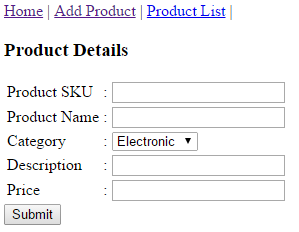
\includegraphics[width=0.6\textwidth]{img/add-product-withCategory}
    \caption{Halaman tambah produk dengan pilihan kategori},
    \label{fig:addProductWithCategory}
\end{figure}

\begin{figure}
    \centering
    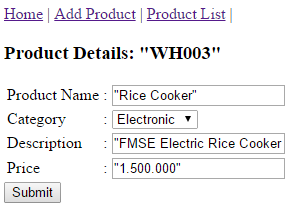
\includegraphics[width=0.6\textwidth]{img/update-product-withCategory}
    \caption{Halaman ubah produk dengan pilihan kategori},
    \label{fig:updateProductWithCategory}
\end{figure}

\begin{figure}
    \centering
    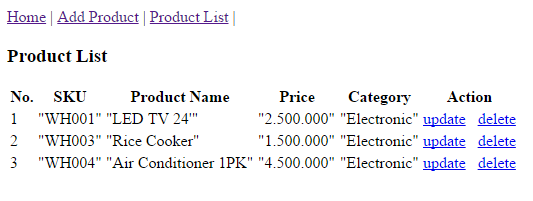
\includegraphics[width=0.8\textwidth]{img/list-product-withCategory}
    \caption{Halaman daftar produk dengan kolom kategori},
    \label{fig:deleteProductWithCategory}
\end{figure}

Sampai pada tahap ini, penulis telah berhasil menerapkan \textit{delta modelling} di dalam ABS MVC Framework yang dapat digunakan untuk menangani perubahan \textit{requirement} pada aplikasi.